% !TEX root = ./../../_Thesis.tex

% subsection's Name and Label
\subsection{Anatomy}
\label{subsec:Anatomy}

The human eye is constituted of several tissues, which contains approximately 126 million receptors cells \cite{King2012}. It can be divided into three concentric layers and two chambers, plus the iris, pupil, and lens. In an adult, it has an average length of 25.4 mm. The outermost layer is the {\it sclera}, the middle layer is the {\it uvea}, and the innermost layer is the {\it retina}. Figure \ref{fig:cross_section} shows a cross section an a human eye and its parts.

\begin{figure}[!t]

	\centering
	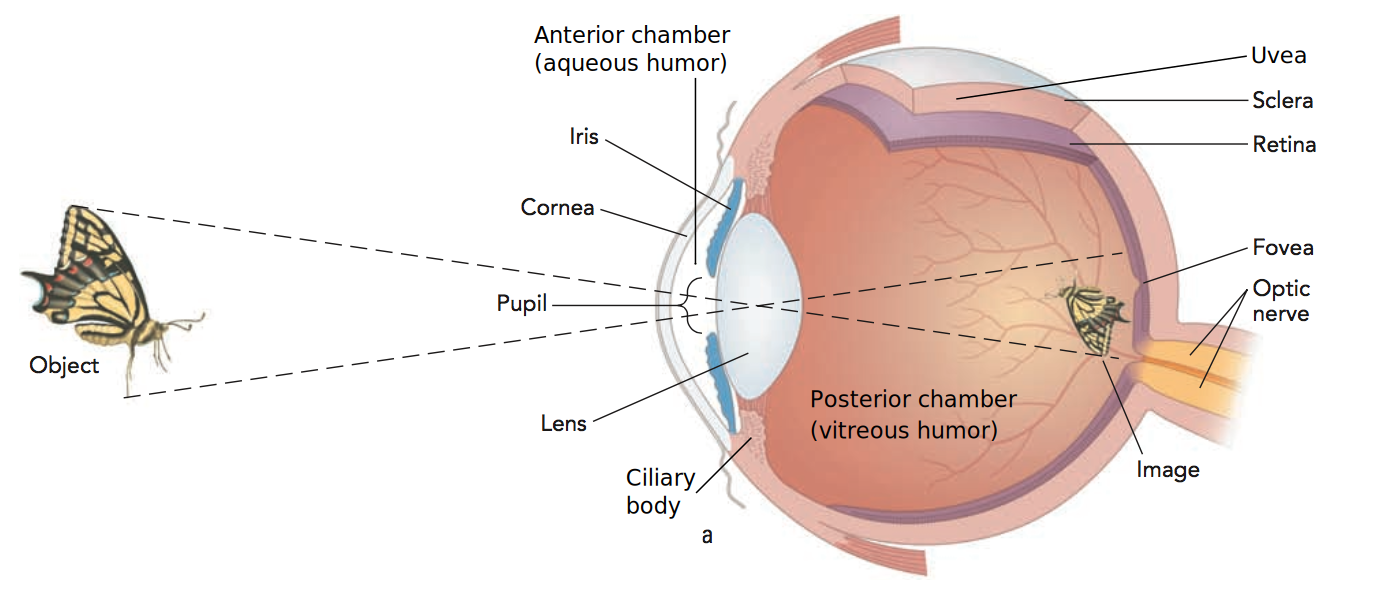
\includegraphics[width=1.00\linewidth]{__Images/02/new-eye.png}
	\caption[Parts of the Eye]{Parts of the Eye. Note that the image of the butterfly on the retina is upside down. The brain allows us to see the image right side up. (modified from \citet{King2012}).}
	\label{fig:cross_section}
\end{figure}

The sclera averages about 1 millimeter in thickness and is made of tightly packed, interwoven fibers that guarantee its toughness. The sclera needs to be tough due to eyeball's pressure, which is the double of the atmospheric pressure \cite{Blake2005}. There is a transparent membrane at the very front of the eye, called {\it cornea}. The cornea is responsible for two-thirds (40 diopters) of the eye's refractive power (total power of 60 diopters) \cite{Tkaczyk2010}. Most part of the uvea layer consists of a heavily pigmented, spongy structure called the {\it choroid}. The choroid averages 0.2 mm thick and contains a network of blood vessels, including capillaries, for blood supply. Its pigmentation reduces light scattering by capturing light that is not captured by the retinal receptor cells. According to \citet{King2012}, the "retina is a light-sensitive surface that records electromagnetic energy and converts it to neural impulses for later processing". It has two kinds of photoreceptors (\ie, light sensitive receptors cells): rods and cones. The retina resembles a very thin, fragile meshwork, which explains its name --- \emph{rete} is Latin for "fisherman's net" \cite{Blake2005}.

Both anterior and posterior chambers contains a specific humor (Figure \ref{fig:cross_section}), which is a transparent liquid continuously produced by the ciliary body. Both aqueous and vitreous humors serve a number of important functions, as maintain the eyeball's shape and nourishment. The iris is the circular section of tissue that gives the eye its characteristic color: brown, blue, green, etc. In the middle of the iris there is 
%a round black region, called pupil. 
the pupil, whose size varies according to the illumination level with the help of two sets of muscles --- the inner and radial \cite{Schwiegerling2004}. Its average diameter varies from 2 millimeters to 8 millimeters, and depends on several factors, such as individual characteristics and luminance level \cite{Yoder2011}.

Right behind the iris, lies an important optical element of the eye, the crystalline lens (see Figure \ref{fig:cross_section}). A gradient-refractive-index lens that contributes approximately one-third (20 diopters) of the dioptric power of the eye, and modifies its shape to focus on near or distant objects \cite{Schwiegerling2004}. This variation, from nearly flat to rounder, causes changes in the final optical power and is called {\it accommodation}. Through accommodation, the lens can correctly focus on the retina the light coming from the scene. For good vision, the crystalline lens must be transparent. %Light must be able to pass through it easily.
Loss of transparency, known as {\it cataracts} leads to a decrease in vision quality
%, called cataracts (\ie, an opacity or reduced transparency of the crystalline lens) 
\cite{Schwartz2010}.